%%
%% 2019 07 04 Ph. G. Freimann
%%

\section{Kreisberechnungen}\index{Kreisberechnungen}\index{Berechnungen am Kreis}
\sectuntertitel{Warum sind Seeräuber so schlecht in Geometrie? --- Weil sie $\pi$ raten!}
%%%%%%%%%%%%%%%%%%%%%%%%%%%%%%%%%%%%%%%%%%%%%%%%%%%%%%%%%%%%%%%%%%%%%%%%%%%%%%%%%


\subsection*{Lernziele}

\begin{itemize}
\item einfache Kreisberechnungen
\item Kreisring
\item Sehne (und Sekante)
\item Segment und Sektor
\end{itemize}

\TadBMTG{56}{4}
\newpage


\subsection{Kreisfläche und Kreisumfang}

\begin{gesetz}{Kreislinie}{}\index{PI@$\pi$ (Pi)}\index{$\pi$}
  Die Länge der Kreislinie wird aus dem Durchmesser $d=2r$  mittels Kreiszahl
  $\pi$ berechnet. Es gilt für den Umfang $U$:
  $$U = 2r\pi = d\pi$$
\end{gesetz}

\begin{gesetz}{Kreisfläche}{}\index{Kreisfläche}
  Die Kreisfläche $A$ eines Kreises mit Radius $r$ wird wie folgt
  berechnet:
  $$A = r^2\pi$$
\end{gesetz}
Herleitung
\TNTeop{Pizza: Schneiden, auslegen = halbe Rechtecksfläche.}

%%%%%%%%%%%%%%%%%%%%%%%%%%%%%%%%%%5
\subsubsection{Kreisringfläche}

\bbwCenterGraphic{8cm}{tals/plani/img/Kreisring.png}

\begin{gesetz}{Kreisring}{}\index{Kreisring}
  Die Kreisringfläche ist die Differenz der umgebenden Kreisfläche
  (Radius $R$) und
  der inneren Kreisfläche (Radius $r$):

  $$A = A(R) - A(r) = R^2\pi - r^2\pi = (R^2-r^2)\pi$$
\end{gesetz}

\begin{bemerkung}{Kreisring}{}
  Die Formel stimmt auch, wenn die Kreismittelpunkte nicht
  übereinstimmen und sich die Kreislinien nicht überlappen (s. Grafik).
  \end{bemerkung}

\subsection*{Aufgaben}

%% Kreisfläche
%%\TALSAadBFWG{43ff (Kreisfläche)}{159. 160. 165. 168.}
\AadBMTG{63}{1., 2. c) d), 4., 10. (Kreisring) und 11. (Kreisberührung)}

\newpage


\subsection{Kreisbogen und -sektor}
\begin{gesetz}{Kreisbogen und
    Kreissektor}{}\index{Kreissektor}\index{Kreisbogen}
  Für den Sektorwinkel $\varphi$ werden Bogen $b$ und Sektorfläche
  $A_{\text{Sektor}}=A_{\text{SK}}$ wie folgt berechnet:
  
  $$b = 2r\pi \cdot{}\frac{\varphi}{360\degre} = r\cdot{} \varphi
  \cdot{} \frac{\pi}{180\degre}= r\cdot{} \stackrel{\frown}{\varphi}$$
  $$A_{\text{SK}} = r^2\pi\cdot{}\frac{\varphi}{360\degre} = \frac12\cdot{}b\cdot{}r$$
\end{gesetz}


Begründung \LoesungsRaumLang{Dreisatz}
\TNT{6}{Bogen: Es gilt das Verhältnis
  $$b : (2r\pi) = \varphi : 360\degre$$

  Analog Fläche:
  $$A_{\text{SK}} : (r^2\pi) = \varphi : 360\degre$$
  $$A_{\text{SK}} \cdot{} 360\degre = r^2\pi\cdot{}\varphi$$
}

\subsection*{Aufgaben}

\AadBMTG{65ff}{12. c), 13. (Bogenmaß) und 14.}

\newpage



\subsection{Kreissegment}

\TRAINER{\bbwCenterGraphic{8cm}{tals/plani/img/Kreissegment.png}}
\noTRAINER{\bbwCenterGraphic{8cm}{tals/plani/img/KreissegmentLeer.png}}

\begin{definition}{Kreissegment}{}
  Wir verwenden die folgenden Notationen:
  \begin{tabular}{ll}
    $r:$        & Radius \\
    $s:$        & Sehne  \\
    $\varphi: $ & Zentriwinkel \\
    $h:$        & Höhe des Segments\\
    $r-h:$      & Höhe des Dreiecks \\
    $A_{SG}:$    & Segmentfläche ($A_{\text{Segment}}$)
    \end{tabular}  
\end{definition}

\begin{gesetz}{Kreissegmentfläche $A_{SG}$}{}
  $$A_{\text{Segment}} = A_{\text{Sektor}} - A_{\text{Dreieck}}$$
  $$A_{SG} = \frac{r^2\pi\varphi}{360\degre} - \frac{s(r-h)}{2}$$
\end{gesetz}
\newpage


\subsubsection{Segmente zusammensetzen}

\begin{bemerkung}{$\varphi>180\degre$}{}
\textbf{Achtung} falls der Zentriwinkel $\varphi > 180\degre$ ist, muss
das Dreieck angefügt werden ...
\begin{center}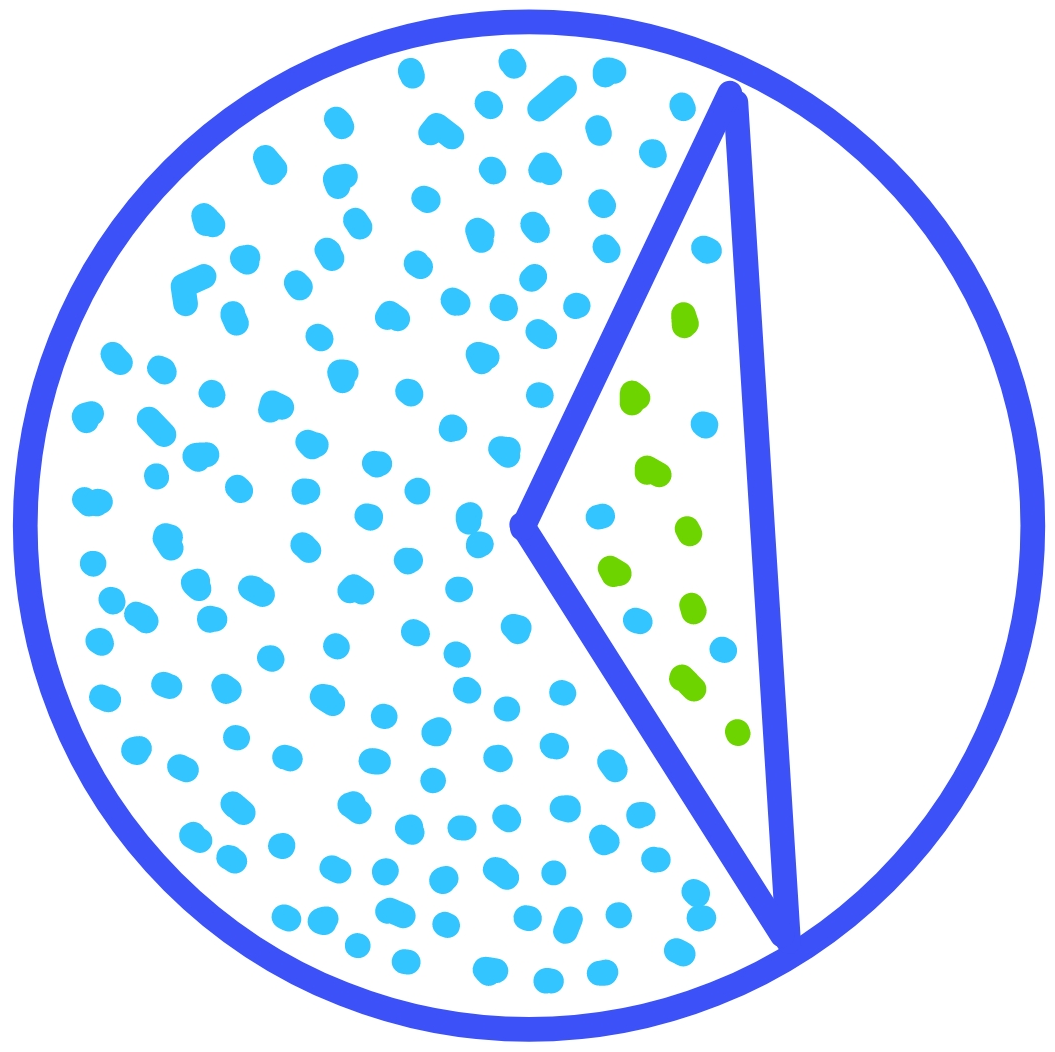
\includegraphics[width=3.5cm]{tals/plani/img/segment_addieren.png}\end{center}
$$A_{\text{SG}} = A_{\text{SK}} \textbf{+} A_{\Delta}$$


... oder das gegenüberliegende Segment wird vom Vollkreis abgezogen:

\begin{center}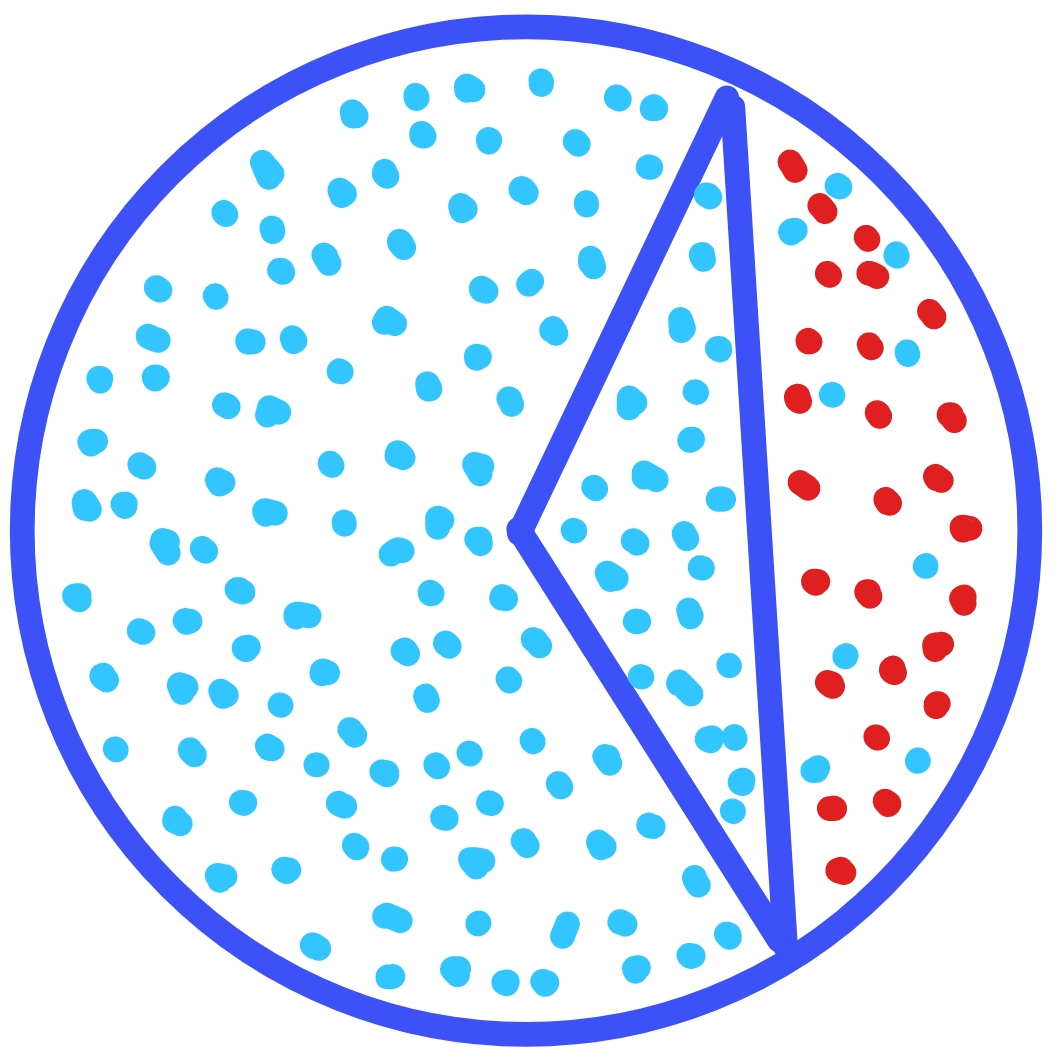
\includegraphics[width=3.5cm]{tals/plani/img/segment_subtrahieren.png}\end{center}
$$A_{\text{SG}}(\varphi) = 2r^2\pi - A_{\text{SG}}(360\degre -\varphi)$$

\end{bemerkung}



\TRAINER{Für das Kreissegment Siehe \cite{marthaler20geom} Seite 61 Kap. 4.2.3.}
\newpage



\subsection*{Aufgaben}

\AadBMTG{123}{39. a) b) c) d)}%% Aufgabe schon vorgelöst
\AadBMTG{66}{15. b) und  17.}
\AadBMTG{38}{15.}
\AadBMTG{39}{29., 30.}
\AadBMTG{41}{36.}


\olatLinkArbeitsblatt{Strukturaufgaben}{https://olat.bbw.ch/auth/RepositoryEntry/572162090/CourseNode/107682599240642}{VT1\_7
  (Segment) und VT1\_8 (Figur)}


%% Kreissektor und Segment
%%\TALSAadBFWG{48ff(Kreissektor)}{179. 180. 183. 185. 187. 188. 189. 192. 194.}



%% Kreissegment
%%\TALSAadBFWG{51ff (Kreissegment)}{197. 198. 200. 204. 206.}


%% Vermischte Aufgaben
%%\TALSAadBFWG{53ff (vermischte Aufgaben)}{209. 215. 219. 223.}
\newpage
